%#####################################################################
%                           Chapter
%#####################################################################

%#####################################################################
\chapter{Implementation Attacks}
\thispagestyle{fancy}
\label{chap:impl_attacks}
%#####################################################################
For a long time, it was believed that designing a mathematically secure algorithm is sufficient to protect the respective cryptographic keys. The cryptographic algorithm was regarded as a black box, i.e., the adversary only knows inputs, outputs, the internal structure, but does not have access to internal, intermediate values. Around~1997 (and in governmental agencies probably much earlier), it was found that this notion is insufficient if the adversary has \emph{physical access} to the cryptographic \ac{DUT}. Techniques like active \acf{FI} and passive \acf{SCA} were shown to be able to break analytically secure ciphers like \ac{DES}, \ac{AES}, and \ac{RSA} in minutes or seconds~\cite{dpa_kocher,BonehDemilloLipton97,timing_kocher}. 

The field of \emph{implementation attacks} comprises a large number of different attack techniques. What all methods have in common is that they exploit properties of the actual implementation, not the mathematical assumptions. For example, for software implementations, \emph{buffer overflows} are an implementation attack: Even if the implemented cipher is secure, a buffer overflow that allows to directly read cryptographic keys renders the security assumptions invalid. 

In the field of embedded systems and hardware, implementation attacks are often based on measuring or manipulating physical properties, e.g., recording the power consumption, inducing faults during computations, and so on. We will focus on these two types of implementation attacks. However, note that other classes (e.g., software vulnerabilities like buffer overflows) are equally important for embedded systems.

\section{\acl{FI}}
Every computing device (and especially \acp{muC}) requires certain conditions to function normally and compute correct results. These include:

\begin{itemize}
	\item A stable supply voltage (typically 3.3\,V, 1.8\,V, or 5\,V in older systems),
	\item a stable clock signal (often supplied by an external oscillator),
	\item ``normal'' operating temperature (usually between -15$\degree$\,C and 80$\degree$\,C),
	\item no strong magnetic or electric fields in the vicinity, and many more conditions.
\end{itemize}

If one or more of these conditions are not met, the device may start to return incorrect results. For instance, memory reads or writes could fail, arithmetic operations return incorrect results, conditional jumps not be executed, and so on. An adversary can hence induce such \emph{faults} on purpose, for example, with one of the following methods:

\begin{itemize}
  \item Expose the device to high or low temperatures. Since temperature changes slowly, this will have effects for longer amounts of time. It could for example reduce the entropy of a \ac{RNG} or disable memory writes. 
	
	\item Manipulate the supply voltage to expose the device to short overvoltages (``pulses'') and undervoltages (``glitches''). If precisely timed, this can affect a single or a few instructions.
	
	\item Temporarily increase the clock frequency (or change the clock signal shape) to overclock the device for a short period. Similar to the supply voltage, this can have effects on the instruction level.
	
	\item Open the \ac{IC} package and and expose the circuit to \ac{UVC} light. This can for example clear Flash and \ac{EEPROM} memory. Aternatively, a photo flash can have similar effects.
	
	\item Open the \ac{IC} package and target specific parts of the circuitry with a focused laser beam. This allows modifications of single signals within the target device (e.g., a single memory location or a single bit of a data bus) with sub-instruction precision. However, the necessary equipment is much more expensive than for the above techniques.
	
	\item Use so-called microprobes to tap and change internal signals on the opened \ac{IC}. For example, cryptographic keys could just be read from memory, or internal signals be changed precisely. Another possibility is the use of a so-called \ac{FIB} to change the \ac{IC} structures on a microscopic level. However, this requires extremely expensive equipment usually only found in high-end semiconductor test labs.
\end{itemize}

Note that the above list is by far not exhaustive. A good overview is given in~\cite{Hamid04thesorcerers}.

\subsection{Generic \acs{FI} Attacks}
There are certain \ac{FI} attacks that are general, i.e., apply to every cipher. An easy-to-grasp example is the skipping of an operation. Take the following example of a PIN comparison:

\lstset{language=C}
\begin{lstlisting}
int c = memcmp(entered_pin, stored_pin, pin_len);

if(c != 0)
{
   return -1;
}

// Code continues ...
\end{lstlisting}

Assume a fault can be induced with instruction-level precision, then, the adversary can simply skip the ``return -1;'' in the \verb+if+ condition and bypass the PIN check. Similarly, it could be possible to bypass a signature verification, a \ac{MAC} check, and so on.

A different generic attack~\cite{BihamShamir97} assumes the following \emph{fault model}: a fault induced on a single bit always sets the bit to zero, i.e., a 1 is turned into a 0, a 0 stays at 0 (``stuck-at'' fault). Furthermore assume that the adversary can selectively fault each single bit of cryptographic key during the load. 
Let $e_k$ be a cipher with $m$-bit key $k$, and $\overline{e}_k^{(i)}$ indicate the cipher where a fault has been induced for the $i$th key bit.
Then, the adversary recovers the full key as follows:

\begin{algorithm}
\center
\begin{algorithmic}
\vspace{2mm}

\State Pick any plaintext $p$
\State $c_{ref} \gets e_k\left(p\right)$
\vspace{2mm}
\For{$i = 0 \ldots m - 1$}
\vspace{1mm}
	\State $c \gets \overline{e}_k^{(i)}\left(p\right)$
	\If{$c = c_{ref}$}
		\State Key bit $i$ is 0
	\Else
	  \State Key bit $i$ is 1
	\EndIf
	\vspace{1mm} 
\EndFor
\vspace{2mm}
\end{algorithmic}
\caption{General fault attack with ``stuck-at'' fault model}
\label{alg:impl_attacks:gen_fi}
\end{algorithm}

The attack of Algorithm~\ref{alg:impl_attacks:gen_fi} works because the adversary can see if faulting a single bit has an effect on the ciphertext. If the ciphertext changed compared to the correct one $c_{ref}$, he concludes that the key bit was 1 (fault changed a 1 to a 0). Otherwise, the fault left a 0 at 0, and the ciphertext is unchanged. 

Both generic attacks require significant control over the fault and its location in time and ``space''. In the following subsection, we look at attacks tailored to specific ciphers, hence requiring less control over the fault parameters.

\subsection{\acs{FI} on \acs{CRT}-\acs{RSA}}
The attacks presented in this section are amongst the earliest reported fault attacks~\cite{BonehDemilloLipton97}. The attack is commonly to referred as ``Bellcore'' attack (due to the affiliation of the authors), and an improvement by Arjen~Lenstra as the ``Lenstra'' attack. Both target \ac{RSA} with a very common optimization based on the \ac{CRT}. Before we describe the attack, we briefly explain this optimization.

\paragraph{\acs{RSA} with \acs{CRT}} 
The \acl{CRT} allows to split one \ac{RSA} computation modulo the $k$-digit number $n$ (e.g., signature generation $s = x^d \mod n$) into two operations modulo $p$ and $q$. Both $p$ and $q$ have approximately half the bit length of $n$, i.e., are $\nicefrac{k}{2}$ digits long. The algorithm to compute $s = x^d \mod n$ (or equally decryption) works as described in Algorithm~\ref{alg:impl_attacks:rsa_crt}.

\begin{algorithm}
\center
\begin{algorithmic}
\vspace{2mm}

\State The following quantities are pre-computed once:
\State $d_p \gets d \mod p-1$
\State $d_q \gets d \mod q-1$
\State $c_p \gets q^{-1} \mod p$
\State $c_q \gets p^{-1} \mod q$
\vspace{2mm}

\State Then, compute:
\State $x_p \gets x \mod p$
\State $x_q \gets x \mod q$
\State $s_p \gets x_p^{d_p} \mod p$
\State $s_q \gets x_q^{d_q} \mod q$
\vspace{2mm}

\State Recombine result:
\State $s \gets \left[q \cdot c_p\right] \cdot s_p + \left[p \cdot c_q\right] \cdot s_q \mod n$

\vspace{2mm}
\end{algorithmic}
\caption{\ac{CRT}-\ac{RSA} signature computation}
\label{alg:impl_attacks:rsa_crt}
\end{algorithm}

To understand the advantage of this approach, recall from Section~\ref{sec:asymmetric_crypto:mul} that multiplication has complexity $\bigo{\left(k^2\right)}$, and that the \ac{SAM} algorithm takes approximately 1.5\,$\ell$ multiplications for an $\ell$ bit exponent. Hence, for the normal computation, we have $1.5\, \ell\,k^2$. For the \ac{CRT} optimization, we need two modular exponentiations with half the bit length for operands and exponent. Hence, we have complexity

$$2 \cdot 1.5\, \frac{\ell}{2}\,\left(\frac{k}{2}\right)^2 = \frac{1.5}{4}\,\ell\,k^2$$

In other words, the \ac{CRT} allows us to reduce the computational complexity by a factor of \emph{four}, neglecting the (minor) efforts for splitting the input and recombining the result. This is why it is very common especially in constrained embedded devices.

\paragraph{Bellcore Attack}
The fault model for the Bellcore attack is very relaxed: We assume that the adversary can inject any fault into the computation $s_p = x_p^{d_p}$ (or equivalently $s_q = x_q^{d_q}$). Then given a correct signature $s$ and a faulty signature $\overline{s}$, the modulus $n$ can be factored with high probability as follows:
$$
q = \mbox{gcd}\left(s - \overline{s},\,n\right),\, p = \frac{n}{q}
$$

The reason why this works is given in the following equation:

$$
s - \overline{s} = \left[q \cdot c_p\right] \cdot s_p + \left[p \cdot c_q\right] \cdot s_q - \left[q \cdot c_p\right] \cdot \overline{s_p} - \left[p \cdot c_q\right] \cdot s_q = q \cdot c_p \cdot \left(s_p - \overline{s_p} \right) \nonumber\\
                 = \lambda\,q
$$

i.e., we get a multiple of $q$ for which $\lambda \neq p$ almost always. Hence, $\mbox{gcd}\left(\lambda\,q,\,p \cdot q\right) = q$.

\paragraph{Lenstra Attack}
The ``disadvantage'' of the  Bellcore attack is that it requires a correct and a faulty signature on the same plaintext $x$. Thus, if the adversary cannot control the input to the signature, e.g., due to randomization, the attack does not work. However, Lenstra's improvement allows to apply the attack by ``emulating'' the correct value using signature verification. More precisely, assume we have a faulty signature $\overline{s}$ as above and the corresponding plaintext $x$. Then, note that (since the fault was induced on $s_p$), the result is still correct modulo $q$, i.e.,
$$
\overline{s} \mod q = \left[p \cdot c_q\right] \cdot s_q = s \mod q
$$
In other words, if we ``verify'' the signature modulo $q$, we have
$$
\overline{s}^e \mod q = s^e \mod q = x \mod q
$$
Thus, in general (not modulo $q$), we have
$$
\overline{s}^e = x + \delta \cdot q\ \Leftrightarrow\ \overline{s}^e - x = \delta \cdot q
$$
with $\delta \neq p$ with high probability, i.e., again a multiple of $q$. Thus, we can again factor:
$$
q = \mbox{gcd}\left(\overline{s}^e - x,\,n\right),\, p = \frac{n}{q}
$$

%\paragraph{Example} Assume $p = 13$, $q = 17$, $n = 221$, $e = 7$, $d = e^{-1} \mod 12 \cdot 16 = \mod 192$, 


%\subsection{\acs{FI} on Symmetric Ciphers: \acs{AES}}

\subsection{Countermeasures}
Countermeasures against fault attacks can be generally divided into two classes: general \emph{detection-based} and \emph{algorithmic} approaches. Detection-based countermeasures are often implemented on the hardware or a low software level and aim to detect that \ac{FI} is taking or has taken place, independent of the specific algorithm. Examples for this include:

\begin{itemize}
	\item Monitoring of power supply and clock signal for glitches,
	\item monitoring of environmental conditions like temperature, 
	\item use of sensors to detect light and laser \ac{FI},
	\item redundant computations, e.g., with two identical \acp{CPU} in parallel or two times subsequently,
	\item insertion of checks into program code to ensure that the control flow is not manipulated, and
	\item checksums and partity bits on internal signals and the data bus.
\end{itemize}

In contrast, algorithmic countermeasures make use of certain properties of a specific algorithm (e.g., \ac{RSA} or \ac{AES}) to detect faults. These include:

\begin{itemize}
	\item ``Infective computations''~\cite{CIA10} to render faulty results useless,
	\item computation of an algorithm and its inverse, e.g., directly verifying an \ac{RSA} signature or decrypting an \ac{AES} ciphertext before outputting it,
	\item additional, more efficient checks like an approach patented by Shamir, see e.g.~\cite{joye2009protecting}, and
	\item insertion of dummy operations to make it harder to inject a fault at a specific position.
\end{itemize}

Note that the above lists are by far not complete---numerous research papers have been published in the area of \ac{FI} countermeasures since around 1997. 
The question arises how an embedded device should react on detection of a potential fault. This of course depends very much on the application and the required level of security. For instance, a high-security smartcard may completely seize to function after a relatively low number of faults have been detected. On the other hand, a device with high reliability requirements (e.g., an automotive \ac{ECU}) may continue to work even if potentially intentional faults occur, but for example block the access to cryptographic operations for some time or at least log the incident.

A cautionary note on counters for counting \ac{FI} attempts: first of all, such counters require some form of permanent memory (e.g., Flash or \ac{EEPROM}), that is not always available. Secondly, writes to such memories can be usually observed in the power consumption or other side channels (see Section~\ref{sec:impl_attacks:sca}). Hence, care must be taken how such counters are incremented. The most obvious approach of incrementing the counter after the detection of \ac{FI} enables the following attack:

An adversary injects a fault, and observes whether a memory write is about to occur (i.e., the counter is incremented). If this is the case, he removes the power from the target device to prevent the memory write. Then, he slightly adjusts his \ac{FI} parameters (e.g., aim laser at a different location, reduce amount of voltage glitch or pulse, change moment in time, etc), and attempts a new \ac{FI}. This renders the use of counters ineffective alltogether.

The correct way for using fault counters would be: On the start of a cryptographic operation to be protected, increment and write the counter. Then, carry out the operation. Only if the operation was successful, decrement the counter again. The main disadvantage is that for \emph{every} invocation of the protected operation, a memory write is now required, which is expensive in terms of power consumption and computation time. In addition, permanent memories like Flash and \ac{EEPROM} have limited write cycles (in the range of 10,000 \ldots 1,000,000 cycles). However, new memory technologies (like \ac{FRAM} used in the MSP430 variant used for this lecture) may help to solve this problem, since they offer permanent storage at little additional cost and have virtually unlimited write cycles.

\section{\acl{SCA}}
\label{sec:impl_attacks:sca}
\acf{SCA} is based on the passive measurement of physical properties of an implementation while it performs cryptographic operations. The side-channel signal or leakage is usually called \emph{trace}. Examples for some of the most common side channels include:

\begin{description}
	\item[Execution time] The execution time or ``timing'' may leak information on secret data, for example through different code branches~\cite{timing_kocher} being taken or through cache-timing side channels~\cite{bernstein2005cache}.
	
	\item[Power consumption] The power (or rather current) consumption of an \ac{IC} depends on the processed data. This is probably the most classical side channel and was introduced by Kocher et~al.~around~1996~\cite{dpa_kocher}.
	
	\item[\ac{EM} emanation] The \ac{EM} emanation~\cite{AgrawalARR02} of an \ac{IC} can give information equivalent to the power consumption, but also allow very detailed, localized measurements of single circuit components. 
	
	\item[Photonic emissions] The photonic emissions (recorded with a microscope and an infrared-sensitive camera) of an opened \ac{IC} can yield a very precise picture of the internal processes, down to the bit level~\cite{aesBlinks,Schl12}.
	
	\item[Sound] The high-frequency sound due to vibrating circuit components can leak information especially for slow algorithms like \ac{RSA}~\cite{acoustic_sca_rsa}.
\end{description}

\begin{figure}[h!tb]
		\center
		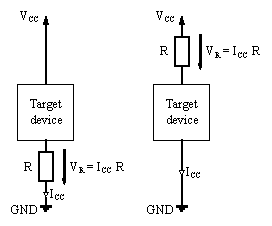
\includegraphics[width=0.5\textwidth]{figures/impl_attacks/measurement}	
		\caption{Typical measurement setup for power consumption side-channel attacks}
		\label{fig:impl_attacks:measurement}
\end{figure} 


\paragraph{Measurement Setup}
Figure~\ref{fig:impl_attacks:measurement} shows the two most typical setups for measuring the power (current) consumption of a target device. In the left setup, a (small) shunt resistor $R$\footnote{usually between 1\,$\Upomega$ and several hundred $\Upomega$} is inserted into the ground path of the target device. Since the supply current $I_{CC}$ flows through the resistor, it can be derived by measuring the voltage drop $V_R$ over $R$ as $I_{CC} = \frac{V_R}{R}$. Note that in \ac{SCA}, usually, we are not interested in the absolute value of $I_{CC}$, but rather require only a value proportional to it. Hence, in practice, one can just measure $V_R$ with a \ac{DSO} and ignore the conversion factor $R$. 

An alternative approach is to place $R$ into the $V_{CC}$ path and again measure the drop over $V_R$. Since $I_{CC}$ is the same for both paths, this approach is equivalent to measuring in the ground path (if there is only one supply voltage). However, when attaching a standard \ac{DSO} probe to measure $V_R$ in the $V_{CC}$ path, note that one obtains $V_{CC} - V_R$, i.e., the signal is \acs{DC}-shifted. Hence, one has to remove the constant \acs{DC} component by measuring \acs{AC}-coupled. Alternatively, $V_R$ can be directly measured using a so-called differential probe. 


%\subsection{Timing}

\subsection{\acl{SPA}}
\acf{SPA} is an umbrella term for side-channel attacks that work by (visually) inspecting one or a few traces. For instance, take the \ac{SAM} (Algorithm~\ref{alg:asymmetric_crypto:ln_sam}): if an adversary can distinguish squaring (SQ) and multiply (MUL), he can trivially reconstruct the secret exponent bit-by-bit. Take the example of the trace in Figure~\ref{fig:impl_attacks:spa_rsa}: The executed operation sequence is: SQ, MUL, SQ, MUL, SQ, SQ, SQ, MUL, SQ, SQ, MUL. 

\begin{figure}[h!tb]
		\center
		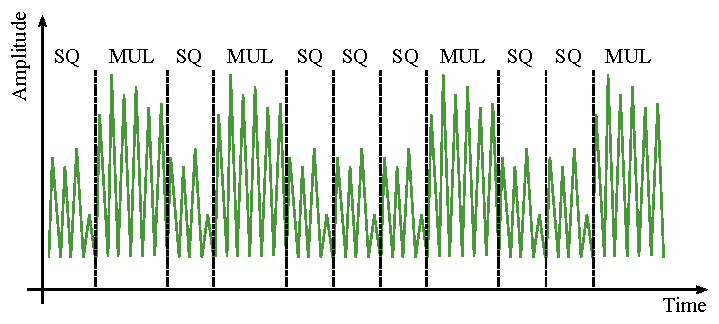
\includegraphics[width=0.7\textwidth]{figures/impl_attacks/spa_rsa}	
		\caption{\ac{SPA} of \ac{SAM} algorithm for \ac{RSA} signature}
		\label{fig:impl_attacks:spa_rsa}
\end{figure} 

\subsection{\acl{DPA}}
\label{sec:impl_attacks:dpa}
While \ac{SPA} attacks utilize larger amounts of side-channel leakage (e.g., of a long-number multiplication consuming many cycles), \acf{DPA}~\cite{dpa_kocher} can exploit tiny leakages (e.g., of a single bit being processed on a large \ac{IC}). To this end, \ac{DPA} uses statistical methods to detect the tiny leakage signal in a larger amount of (noisy) traces. The core assumption of \ac{DPA} is that the power consumption (or other side-channel signals) are slightly different if the target device processes a zero bit or a one bit. However, in contrast to \ac{SPA}, this difference does not have to be ``visible'' and further can be hidden in noise.

A typical \ac{DPA} is divided into two steps, the measurement and evaluation phase, which are described in the following.

\paragraph{Measurement}
\ac{DPA} operates on a set of $n$ traces $p_i \left( t \right)$ with $T$ sample points each (i.e., $t = 0\,\ldots\,T-1$). Each trace is the power consumption while the target device encrypts a plaintext $X_i$ (or performs another cryptographic operation) using the key $k$. In the following, when we talk about bytes (or other parts) of $x_i$, we will use the notation $X_i^0$ to for example denote byte~0 of $X_i$. If it is clear from the context that we only talk about a specific byte, we write $x_i$. The measurement phase is summarized in Algorithm~\ref{alg:impl_attacks:dpa_measure}.

\begin{algorithm}
\center
\begin{algorithmic}
\vspace{2mm}

\For{$i = 0  \ldots n-1$}
	\State Generate random, uniformly distributed plaintext $X_i$
	\State Send $X_i$ to device, device computes $enc_K \left(X_i \right)$
	\State Measure power consumption $p_i\left(t\right)$
	\State Store $p_i\left(t\right)$ and corresponding $X_i$
\EndFor

\vspace{2mm}
\end{algorithmic}
\caption{Measurement phase of a \ac{DPA}}
\label{alg:impl_attacks:dpa_measure}
\end{algorithm}

\paragraph{Evaluation}


The evaluation process (for the first byte/part $k$ of the round key) for the example of the \ac{AES} is summarized in Algorithm~\ref{alg:impl_attacks:dpa_eval}.

\begin{algorithm}[h!tb]
\center
\begin{algorithmic}
\vspace{2mm}

\State $S_{0}^{\hat{k}}\left(t\right) \gets\ $  empty set for each candidate $\hat{k}$ for $k$
\State $S_{1}^{\hat{k}}\left(t\right) \gets\ $  empty set for each candidate $\hat{k}$ for $k$
\vspace{2mm}
\For{$i = 0  \ldots n-1$}
	\vspace{1mm}
	\State Load trace $p_i\left(t\right)$ and plaintext $X_i$
	\State $x_i \gets\ $ first byte/part of $X_i$
	\vspace{1mm}
	\For{$\hat{k} = 0 \ldots 255$}
		\vspace{1mm}
		\State $b \gets S\left(x_i\,\oplus\,\hat{k}\right)$
		\If{$\mbox{LSBit}\left(b\right) = 0$}
			\State Add $p_i\left(t\right)$ to $S_{0}^{\hat{k}}$
		\Else
			\State Add $p_i\left(t\right)$ to $S_{1}^{\hat{k}}$
		\EndIf
	\EndFor
	\vspace{1mm}	
\EndFor
\vspace{2mm}
\For{$\hat{k} = 0 \ldots 255$}
	\vspace{2mm}
	\State $\overline{S}_{0}^{\hat{k}}\left(t\right) \gets \frac{1}{\left|S_{0}^{\hat{k}}\right|} \sum_{p_i \in S_{0}^{\hat{k}}}{p_i\left(t\right) }$
	\State  $\overline{S}_{1}^{\hat{k}}\left(t\right) \gets \frac{1}{\left|S_{1}^{\hat{k}}\right|} \sum_{p_i \in S_{1}^{\hat{k}}}{p_i\left(t\right) }$
	\vspace{2mm}
	\State $\mbox{DPA}^{\hat{k}}\left(t\right) \gets \overline{S}_{1}^{\hat{k}}\left(t\right) - \overline{S}_{0}^{\hat{k}}\left(t\right)$
\vspace{2mm}
\EndFor
\vspace{2mm}
\State Find $\mbox{DPA}^{\hat{k}}$ with highest peak to recover $k = \hat{k}$.

\end{algorithmic}
\caption{Evaluation phase of a \ac{DPA} for first byte of \ac{AES}}
\label{alg:impl_attacks:dpa_eval}
\end{algorithm}

\paragraph{Why \acs{DPA} works}
\ac{DPA} apparently allows to target the leakage of a single bit of a single register or memory location in a potentially very large circuit. The question arises why this approach works. The main reason is that we \emph{average} many signals, which reduces the amount of noise relatively to the signal (i.e., the leakage of a single bit). More precisely, we can write a power trace at a point in time $t_0$ as 

$$p\left(t_0\right) = p_{signal} + \mathcal{N}_{alg} + \mathcal{N}_{measure}$$

where $p_{signal}$ is the actual leakage, $\mathcal{N}_{alg}$ algorithmic noise (caused by all the parts of the circuit we do not predict), and $\mathcal{N}_{measure}$ measurement noise (i.e., physical effects in the setup etc.). Assuming $\mathcal{N}_{alg}$, $\mathcal{N}_{measure}$ are Gaussian, for $n \rightarrow \infty$, the noise vanishes and we only see the differences between $p_{signal}$ (bit = 0 and bit = 1) in the difference of means. In practice, $n \rightarrow \infty$ can mean anything between a few ten to millions or billions of traces.

\subsection{\acl{CPA}}
In a \ac{DPA}, we focus on a single bit, while we actually predict more information (e.g., 8~bit for the AES). To make use of this fact and reduce the number of required traces, \acf{CPA}~\cite{Brie04} makes use of a \emph{leakage model}---i.e., the fact that we can approximate how an internal value $b$ affects the leakage signal $p_{signal}$. Figure~\ref{fig:impl_attacks:dpa_signal} shows an example how a single byte could leak: internal values with a lower number of ones result in a lower amplitude, while more ones lead to higher values.

This leakage model is the \ac{HW} model: the side-channel signal is proportional to the \ac{HW} of the processed value, i.e., we have $p_{signal} \propto \mbox{HW} \left(b\right)$. As a reminder, $\mbox{HW} \left(b\right)$ is defined as the number of bits set to~1 in $b$. For instance, $\mbox{HW} \left(0x00\right) = 0$, $\mbox{HW}\left(0xAB\right) = \mbox{HW}\left(10101011\right) = 5$, and $\mbox{HW} \left(0xFF\right) = 8$.

\begin{figure}[h!tb]
		\center
		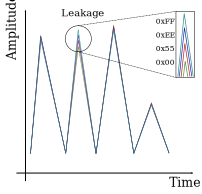
\includegraphics[width=0.4\textwidth]{figures/impl_attacks/dpa_signal}	
		\caption{Leakage of a single byte value $b$}
		\label{fig:impl_attacks:dpa_signal}
\end{figure} 

There are many other conceivable leakage models, the most prominent one being the \ac{HD} model, that assumes that the leakage depends on the \emph{previous} value $b'$ and the \emph{new} value $b$ of a register. The \ac{HD} is the number of bits that have changed between $b'$ and $b$, i.e., $\mbox{HD}\left(b',\,b\right) = \mbox{HW}\left(b'\, \oplus\,b\right)$.

In the following, we use notation based on Section~\ref{sec:impl_attacks:dpa} to explain how \ac{CPA} allows to include the leakage model into an approach similar to \ac{DPA}. Again, we have $n$ traces $p_i \left( t \right)$ with $T$ sample points each and the corresponding plaintexts $X_i$. 
Again, take the example of the \ac{AES} and assume a key candidate $\hat{k}$ for the first \ac{SBOX} with input byte $x_i$. Then, we predict the intermediate value as:

$$
b_{i,\hat{k}} \gets S\left(x_i\,\oplus\,\hat{k}\right)
$$
\vspace{-1mm}

Now, we employ our leakage model $f\left(\cdot\right)$ to convert this value into a hypothetical power consumption (e.g., using the \ac{HW} model): 

$$
h_{i,\hat{k}} = f \left(b_{i,\hat{k}}\right) \stackrel{\mbox{\tiny e.g.}}{=} \mbox{HW}\left( b_{i,\hat{k}}\right)
$$
\vspace{-1mm}

The final step is to determine the ``match'' between the predictions $h_{i,\hat{k}}$ for a key candidate and the reality of the traces $p_i \left( t \right)$. To this end, we use \emph{Pearson's correlation coefficient}~$\rho$, cf.~\cite{wiki:Pearson}. $\rho$ estimates the linear correlation between two data sets $A_i$ and $B_i$: if they are perfectly correlated, $\rho = 1$ and one data set can be written as a linear function $A_i = \alpha \cdot B_i + \beta$ of the other. If there is no correlation, $\rho = 0$. For perfectly inverse-correlated data sets, $\rho = -1$. 
In summary, keep in mind that $-1 \leq \rho \leq 1$.

In our case, one data series is the set of traces $p_i \left( t \right)$, the other one the prediction $h_{i,\hat{k}}$. Since $p_i \left( t \right)$, we compute the correlation point-wise for each time sample. However, note that $h_{i,\hat{k}}$ is not time-dependent, hence, this data series is always the same for all $t$.

Thus, given a key candidate $\hat{k}$, we obtain:

$$
\rho_{\hat{k}}\left(t\right) = \frac{\sum\limits_{i = 0}^{n-1} {\left( h_{i,\hat{k}} - \overline{h}_{\hat{k}}  \right) \cdot \left( p_{i}\left(t\right) - \overline{p}\left(t\right) \right)} }   {\sqrt{\sum\limits_{i = 0}^{n-1} {\left( h_{i,\hat{k}} - \overline{h}_{\hat{k}}\right)^2}\ \cdot \ \sum\limits_{i = 0}^{n-1} {\left( p_{i}\left(t\right) - \overline{p}\left(t\right)\right)^2 }   }} = \frac{\mbox{cov} \left(h_{i,\hat{k}}, p_i\left(t\right)\right)}{\sqrt{\mbox{var}\left(h_{i,\hat{k}}\right) \cdot \mbox{var}\left(p_i\left(t\right)\right)}}
$$

$\rho_{\hat{k}}\left(t\right)$ is the equivalent to the difference-of-means curve $\mbox{DPA}^{\hat{k}}\left(t\right)$ in a \ac{DPA}---the correlation with the highest peak identifies the correct key candidate.

\paragraph{Rules of Thumb} 
In contrast to \ac{DPA}, where the value of a peak in the difference-of-means is hard to predict, \ac{CPA} is normalized to the range $-1 \leq \rho \leq 1$, which makes it easier to define what a \emph{significant} correlation is. \cite{MangardOP_DPABook_07} provides several ``rules of thumb'' for the correlation coefficient.
First, for $n$ traces, the expected ``noise level'' $\rho$ is

$$
\rho_{noise} = \frac{4}{\sqrt{n}}
$$

That means that any correlation $\leq \rho_{noise}$ is essentially meaningless and not significant. This formula reflects the fact that for more traces, it is possible to identify smaller correlations. The second rule of thumb allows to estimate the minimum number of required traces $n_{min}$ to unambiguously extract a key (with very high probability) when the respective correlation for the correct key $\rho_{key}$ is known (e.g., from prior experiments). 

$$
n_{min} = \frac{28}{\rho_{key}^2}
$$

This formula only holds for $\rho_{key} \leq 0.2$. To give an example: Assume after $n = 2000$ traces, we get $\rho_{key} = 0.1$. Clearly, this correlation is significant since $\rho_{noise} = \nicefrac{4}{\sqrt{2000}} = 0.089$. However, to be able to unambiguously extract the key with that correlation, $n_{min} = \nicefrac{28}{0.1^2} = 2800$~traces would be required.

\section{Countermeasures}
Protecting against \ac{SCA} has been an active area of research since the initial discovery around~2000. Hence, we can only look at a small selection of countermeasures in this section. A deeper survey for block ciphers is for example given in~\cite{prouff_ches2013}. Countermeasures to directly thwart \ac{SCA} can be realized on two dimensions (and a combination of them): the amplitude of the leakage and the timing. In addition, countermeasures on the system level can be taken to limit the consequences of successful \ac{SCA}, rather than preventing the actual attack. We will consider examples for all three approaches in this section.

\subsection{Amplitude-based Countermeasures}
The \ac{SNR} determines the success rate of a side-channel attack---the lower the \ac{SNR}, the more measurements will be needed in general. 

\paragraph{Balanced Logic Styles}
A first way to reduce the \ac{SNR} is to reduce the power of the leakage signal by balancing the power consumption. As a simple example, assume all results are computed on differential signals (i.e., a bit $a$ and the complement $\overline{a}$ are always used at the same time). Then, ideally, the leakage should vanish: For example, assuming a \ac{HW} model, we would always observe $\mbox{HW}\left(a\right) + \mbox{HW}\left(\overline{a}\right) = \mbox{const}$, independent of the value of $a$. There is a variety of such balanced logic styles\footnote{For a good overview, cf.~e.g.~\url{https://www.cosic.esat.kuleuven.be/ecrypt/courses/albena11/slides/amir_moradi_secure_logic_styles.pdf}}. However, due to various effects in real \acp{IC} (different routing delays, capacitance, process variations in general), the countermeasures can never fully remove the side-channel leakage. Yet, they help to make \ac{SCA}, especially in combination with other countermeasures, much more difficult.

Another (rather obvious) example for a countermeasure based on reducing the information in the signal is protection against \ac{SPA}, for example for \ac{SAM}-like algorithms. Instead of using a specific implementation for squaring that produces a distinguishable pattern, multiplication can be used for both operations. However, a squaring realized with multiplication may still be recognizable, e.g., because of different memory access patterns. One solution is to use a Square-and-Multiply-always approach, where the result of the multiplication is discarded if the current exponent bit is zero. Other, more refined algorithms like the Montgomery ladder~\cite{montgomery1987speeding} ensure that the same number of squares and multiplications is executed (independent of the exponent) by using two result registers. Note however that \ac{SPA}-protected algorithms are usually still vulnerable to \ac{DPA}.

\paragraph{Noise Generation}
Reducing the \ac{SNR} can alternatively be achieved by increasing the amount of noise. A hardware or software-based noise generator can be used for this purpose, but it should be noted that averaging will allow the adversary to remove this noise again. In other words, noise generation (when used as the only countermeasure) will only increase the number of required traces. However, in combination with other countermeasures (e.g.~randomized timing, see below), it can severely impede \ac{SCA}, for example, because an adversary can no longer re-align traces in time based on signal patterns.

%% Masking
\paragraph{Masking}
Instead of introducing uncorrelated noise or reducing the leakage, \emph{masking} fully randomizes all sensitive internal variables by internally generating a fresh, random mask for each execution of an algorithm. Then, the device only leaks the masked values, which an adversary cannot predict since the mask never ``leaves'' the device. An early description of such a method can e.g.~be found in~\cite{chari1999towards}.

The general idea is to combine the sensitive value $x$ with a random mask $m$, e.g., using \verb+XOR+. Then, the device performs all computations on $x \oplus m$, and unmasks the result before outputting. For operations that are linear with respect to \verb+XOR+ (e.g., \verb+XOR+ing a round key), applying masking is trivial, since for example $\left(x \oplus m\right) \oplus k = \left(x \oplus k\right) \oplus m$.
%
For non-linear components, e.g., an \ac{SBOX} $S$, masking requires to generate a new, masked \ac{SBOX} $S_m$ such that $S_m\left(x \oplus m\right) = S\left(x\right) \oplus m$. In general, the masked \ac{SBOX} depends on $m$ and has to be generated on-the-fly or precomputed for all $m$. However, for specific cases, e.g., the \ac{AES} \ac{SBOX}, algebraic properties can be utilized for more efficient realization~\cite{oswald2005side,canright2008very}.
%
Masking can be understood as being based on secret sharing and multiparty computation, which has lead to newer developments like so-called \emph{threshold implementations}~\cite{nikova2006threshold}.

From the attacker's point of view, masking schemes can be attacked in various ways: first of all, if the random mask $m$ is biased, attacks may still succeed with a larger number of traces. Furthermore, \emph{higher-order} \ac{SCA} (where multiple sample points are combined to exploit combined leakage of sensitive value and mask) allows to mount \ac{DPA} or \ac{CPA} also for masked implementations~\cite{oswald2006practical}.

\subsection{Timing-based Countermeasures}
In contrast to amplitude-based approaches, timing-based countermeasures lower the \ac{SNR} by spreading the leakage over multiple clock cycles. Again, there are various ways to achieve this goal: 
first, the clock signal can be made unstable on purpose, or even randomly frequency-modulated so that a targeted operation is executed at different points in time for subsequent executions of the algorithm. It should be noted that an adversary may be able to re-align a set of traces, e.g., by extracting the peaks in the traces, using pattern matching, or \acs{FM}-demodulating the traces.

Instead of manipulating the shape of the clock signal, dummy operations (or dummy cycles) can be added to the control flow to ensure that a target intermediate value is handled in different clock cycles for different executions. The dummy operations should obviously be indistinguishable from ``real'' operations, otherwise the adversary may be able to remove them, again using pattern matching techniques. 

A slightly more algorithm-specific approach with similar ideas is to randomly change the order of operations (``shuffling''), e.g., the \ac{SBOX} instances of the \ac{AES}. Of course, this is only possible for operations that have no dependency (e.g., \acp{SBOX} applied byte-wise) or that are commutative (e.g., when \verb+XOR+ing or adding several values). A comprehensive discussion can for example be found in~\cite{veyrat2012shuffling}.

It should be noted that timing-based countermeasures generally linearly reduce the attack efficiency, i.e., if a target sample is spread over $\tau$ samples, then the efficiency decreases by a factor of $\tau$. However, by averaging (integrating) all potential target samples (in the simplest case summing $\tau$ samples), this factor becomes $\sqrt{\tau}$. Hence, in practice, protecting an implementation by time randomization alone would require a very large parameter $\tau$. Therefore, they are usually used in combination with other countermeasures.

As a final note, an equally (or potentially even more) important aspect is the protection against timing attacks that exploit secret-dependent runtime variations. It is mandatory that the cryptographic algorithm itself has constant runtime for any combination of inputs (i.e., usually key and plaintext). Amongst others, bitslicing (Section~\ref{sec:symmetric_crypto:bitslicing}) can be used to achieve this goal. The timing randomization then is applied on top of the constant-runtime algorithm, e.g., by inserting dummy cycles. The entropy for the randomization must be independent of the inputs to the algorithm---otherwise, if input data is used to derive ``randomness'' for countermeasures, a trivial timing vulnerability may be inserted into the algorithm. 

\subsection{System Level Countermeasures}
First and foremost, a central countermeasure on the system level is to \emph{diversify} keys, especially for devices that the adversary may get physical access to. This implies that every device gets a unique key---if an adversary manages to extract this key, only one specific device is affected. 
%
What happens when this principle is not followed can be see by the example of a digital locking system~\cite{crypto_paper_sv,Oswald13_1}. In this case, a symmetric master key was present in every locking cylinder of a complete installation (a very large building complex). By attacking a single lock, the adversary can create a device to unlock any door and access any room in the entire installation. 

This is a typical example of a \ac{SPOF}, where a single successful attack has far-reaching consequences. Incidentally, note that attacks on the hardware level are only one of many ways such a master key could be leaked. Other possibilities include insiders (e.g., displeased or bribed employees), network-level attacks and rootkits (key is stored on a vulnerable computer), or unfortunate accidents (backup coy of key is stored on a decommissioned harddrive).

In contrary, for systems with proper key diversification, this problem can be largely avoided, although in general there will likely remain some valuable secrets, yet these are handled in the backend and can be protected by a variety of countermeasures. For example, in the case of a public transport card, proper key diversification ensured that a successful \ac{SCA} did not scale to the compromise of the entire system, but only affected the targeted card~\cite{OswaldPhD13}.

Note that in other cases, e.g., the protection or encryption of device firmware and bitstreams~\cite{Moradi13,Strobel15,Swierczynski14,actelSca,SCAV4V5}, key diversification is not always applicable. Even if keys are diversified, an adversary who solely wants to extract \ac{IP} (e.g., to clone a device) succeeds if he can break the protection on one single device. In these case, strong classical countermeasures are hence of particular importance.

There is a variety of other possible approaches, some implemented on the actual device, others in the backend. To name a few examples: The backend system of a locking system could check for inconsistent access attempts (e.g., two distant doors were accessed approximately at the same time by the same user) to detect cloned tokens. The same applies to payment systems, where shadow accounts can be used to verify that the balance spent with a particular payment card agrees with the  amount charged by the user. In general, devices which are suspected to have been compromised can be blocked. 
In addition, implementation attacks can be detected (or mitigated) on the side of the device, e.g., by blocking suspicious activities like the acquisition of many side-channel traces (attempt or rate limiting). 

In general, system-level countermeasures strongly depend on the particular application and should hence be seen as a ``second line of defense'', should the traditional countermeasures be overcome.

%---------------------------------------------------------------------




